%! TEX root = ../main.tex

\section{Encuesta subjetiva}
\label{sec:subjetiva}

Al final del período de prueba, cada alumno que forma parte de la muestra
completa una encuesta con $31$ preguntas que se utilizan para validar las
hipótesis, las cuales fueron explicadas en el capítulo~\ref{chap:requerimientos}
y para medir sus apreciaciones sobre otros aspectos de la solución que serán
detallados más adelante en esta sección. 

Las preguntas están agrupadas en dos, el primer grupo cuenta con $27$ preguntas
cerradas, es decir de una sola respuesta en una lista de opciones, el segundo
grupo cuenta con $4$ preguntas abiertas, es decir los encuestados pueden dar
respuestas libres a las preguntas. 

De esta forma, se busca identificar las fortalezas y debilidades de la solución,
además de evaluar la solución en cuanto a factores de exploración,
representación, motivación, inmersión, retroalimentación y pedagogía, de acuerdo
a las apreciaciones de los miembros de la muestra.

\subsection{Muestra}

Cada encuesta es entregada a los $11$ alumnos del universo que acordaron
participar en la prueba y que fueron seleccionados como resultado de la 
\emph{Encuesta de ubicación}, mientras completan la encuesta, un guía está presente
para responder cualquier duda.

La utilización de $11$ alumnos es suficiente, ya que según estudios presentados
en~\cite{nielsen2000}, mientras menos experiencia tengan los sujetos de estudio
con la solución planteada, serán necesarios menos para detectar un gran
porcentaje de errores y fortalezas, y según~\cite{ritch2009}, una base de $10$ a
$12$ es suficiente para obtener resultados estadísticamente válidos.

\subsection{Variables}
\label{sec:variables}
\observacion{Parece haber tanta referencia como para separar}

A continuación se describen las variables que tienen por objetivo demostrar la
validez de las hipótesis planteadas en este trabajo descritas en el
capítulo~\ref{chap:requerimientos} y la medición de otros aspectos de la
solución relacionados con los objetivos de este trabajo descritos en la
sección~\ref{sec:objetivos_generales}. Estas variables son agrupadas en
factores, los cuales representan aquellos aspectos de la solución propuesta que
buscan ser evaluados.

Cabe volver a resaltar que la medición de estas variables se realizan
exclusivamente de acuerdo a las valoraciones dadas por la muestra en cada uno de
las preguntas que forman parte de la encuesta.

\subsubsection{Exploración}
\label{sec:sub_exploracion}
\observacion{Creo que el nombre es confuso por que parece referirse al tema de
interacción con el entorno}

\observacion{Se podría simplificar el siguiente párrafo} 

Este factor esta \fixme{relacionado}{} con \fixme{la característica}{} que posee
la solución en cuanto a la \fixme{oportunidad}{} que \fixme{brinda}{} al usuario
para \fixme{explorar}{} cada uno de los elementos del entorno simulado
(paciente, herramientas propias del procedimiento). En este sentido, se busca
proveer facilidad de uso, intuitividad y realismo en cuanto a las acciones y
situaciones que se presentan en la solución para que de esta manera, los
elementos que la componen no representen para el jugador un obstáculo que impida
su uso.
\observacion{El factor que mide la eficiencia es acaso a explorar el entorno?}

Las variables que miden este aspecto son las siguientes:

\begin{description}

\item[Funciones realizadas por los elementos del juego:] se refiere a la
    correctitud con la que una herramienta o elemento del juego representa las
    funciones que el mismo puede realizar en la vida real, en este sentido, se
    evalúa el realismo con el que es representado tal elemento.

\item[Aleatoriedad para afianzar conocimientos:] se refiere al beneficio que
    puede traer el hecho de que el estado del paciente en el juego sea aleatorio
    en cuanto a la posibilidad que esto brinda al jugador para poner a prueba
    sus conocimientos teóricos.

\item[Aleatoriedad para representar realismo:] se refiere al uso de estados
    aleatorios en el paciente para que de esta forma el procedimiento se asemeje
    mas a una situación real.

\item[Facilidad de uso:] se refiere a lo fácil e intuitivo  que puede ser la
    utilización de los elementos del juego.

\end{description}

\subsubsection{Representación}
\label{sec:sub_representacion}

Este factor esta relacionado con la calidad y suficiencia con la que se
representan los diferentes objetos que son simulados en la solución. La
representación abarca tanto funcionalidad como aspecto del objeto.

De esta manera, se busca permitir al jugador realizar con los objetos las
acciones que requiera para llevar a cabo el procedimiento que se le presente en
la solución, y además, representar estos elementos de la mejor manera posible.

Las variables que miden estos aspectos son las siguientes:

\begin{description}

\item [Respuestas del paciente:] se refiere a la suficiencia de las respuestas 
    motrices, oculares y verbales que realiza el paciente en la escena 
    correspondiente a la valoración de la escala de Glasgow.

\item[Distinción entre los estados del paciente:] se refiere a si los diferentes
    estados del paciente son distinguidos correctamente en el procedimiento de
    valoración de la Escala de Glasgow ya que esto es importante para que el
    jugador pueda diagnosticar correctamente al paciente.

\item[Acciones con las herramientas:] se refiere a si las diferentes acciones que
    pueden realizarse con los elementos o herramientas del juego en un
    determinado procedimiento de enfermería son suficientes para ese
    procedimiento, ya que, debido a las limitaciones de la tecnología estas
    acciones son limitadas.

\end{description}

\subsubsection{Motivación}
\label{sec:sub_motivacion}

Este factor esta relacionado con la importancia de incluir en la solución
aquellas características que son propias de un videojuego convencional. Se
busca conocer el valor de estas características en cuanto a la motivación que
puedan producir en los jugadores tanto para volver a utilizar la solución como
para superarse en cada juego.

Las variables que miden estos aspectos son las siguientes:

\begin{description}

\item[Motivación del puntaje:] se refiere a que tanto motiva al jugador que la
    solución le proporcione un puntaje total al final de cada partida para poder
    mejorar constantemente siendo este puntaje como una evaluación final de todo
    lo que realizo dentro de la partida.

\item[Importancia del puntaje:] se refiere a que tan importante es para un
    jugador que se le proporcione un puntaje total al final de cada partida para
    poder visualizar su rendimiento.

\item[Socialización de los puntajes:] se refiere a si el hecho de que las
    personas del mismo entorno compartan sus puntajes, experiencias y logros en
    las partidas a través de redes sociales pueda ser motivador.

\item[Medición del tiempo:] se refiere a que tanto motiva al
    jugador que la solución le proporcione el tiempo que duro su partida
    sirviendo este tiempo como una evaluación de su precisión a la hora de
    realizar el procedimiento que se le presente.

\end{description} 


\subsubsection{Inmersión}
\label{sec:sub_inmersion}

Este factor esta \fixme{relacionado con el sentimiento}{Percepción?} de formar
parte de la escena. Es decir, se trata de evaluar que tanto un jugador puede
sentir que realmente se encuentra dentro del juego para que de este modo el
pueda entrar en ambiente para realizar los procedimientos que se le presenten en
sus partidas de juego.

Las variables que miden este aspecto son las siguientes:

\begin{description}

\item[Escenografía para entrar en ambiente:] se refiere a la importancia de la
    escenografía de la partida para que el jugador entre en ambiente para
    realizar el procedimiento que se le presente.

\item[Juegos cortos como ayuda para la repetición:] se refiere a si el hecho de
    que los procedimientos presentados en las partidas sean cortos contribuye a
    repetir las partidas varias veces de seguido entrando en un estado de
    inmersión.
    \observacion{El titulo de este punto tiene un ?}

\item[Gráficos en tres dimensiones para entender el entorno:] se refiere a la
    importancia que tiene el uso de gráficos en tres dimensiones para que el
    jugador pueda entender mejor el entorno y las posibles acciones que puede
    realizar.

\item[Realismo a través de ordenes verbales:] se refiere a si el hecho de que la
    solución brinde la posibilidad de que aparezca un menú de ordenes verbales
    en el momento en que el jugador habla hace que la acción de dar ordenes
    verbales se asemeje mas a la realidad.

\item[Simulación como herramienta:] se refiere a si la simulación ayuda al
    jugador a sentirse parte del laboratorio, dando cierto realismo a la escena
    que se le presenta.

\end{description}

\subsubsection{Utilidad}
\label{sec:sub_utilidad}

Este factor está relacionado con el potencial de la solución como herramienta 
de apoyo al proceso de aprendizaje de los estudiantes de enfermería.

Las variables que miden este aspecto son las siguientes: 

\begin{description}
\item[Simulación para complementar el estudio en clase y laboratorio:] se
    refiere a que tanto potencial tienen las herramientas alternativas como la
    simulación pueden complementar a los métodos de aprendizaje tradicionales
    que son el estudio en clase y en el laboratorio.

\item[Simulación como proveedor de facilidades para el estudio:] se refiere a si las
    herramientas alternativas como la solución proveen más facilidades para
    poner en practica los conocimientos con respecto a los demás métodos de
    aprendizaje que son los libros, laboratorios y el campo de practicas.

\item[Interacción con el paciente:] se refiere a si el hecho de que el jugador
    pueda interactuar con un paciente que responde a las acciones del jugador 
    implica una mejora con respecto a otros materiales utilizados en los 
    laboratorios de práctica.

\end{description}

\observacion{Algunos parecen estar fuera de lugar (los que tienen ?)}

\subsubsection{Retroalimentación}
\label{sec:sub_retroalimentacion}

Este factor esta relacionado con la importancia de ofrecer al jugador
información acerca de sus logros y errores de manera tal que el pueda estar
consciente de sus puntos fuertes y sus puntos débiles en los diversos
procedimientos que realice en la solución.

Las variables que miden este aspecto son las siguientes:

\begin{description}[style=unboxed]

\item[Detalles de los pasos realizados incorrectamente:] se refiere a 
    la importancia que tiene para el jugador que la solución no sólo le 
    diga los pasos que realizó de manera incorrecta sino también el por qué 
    de ello.

\item[Retroalimentación suficiente respecto a los pasos realizados:] se refiere 
    a sí son suficientes las justificaciones breves acerca de las causas por las 
    cuales se realizó incorrectamente un paso.

\item[Representación iconográfica de conceptos y acciones en la \Gls{gui}:] 
    se refiere a la suficiencia de mostrar iconos en la interfaz de 
    la solución para representar el estado actual del jugador.

\end{description}

\subsubsection{Pedagogía}
\label{sec:sub_pedagogia}

Este factor esta relacionado a la utilidad y al beneficio que puede traer la
solución para apoyar el aprendizaje del jugador. De esta manera, se busca
obtener la validez real de este tipo de herramientas como aporte al aprendizaje,
proveyendo mas interacción al jugador.

Las variables que miden este aspecto son las siguientes:

\begin{description}

\item[Potencial para memorizar y comprender el procedimiento:] se refiere a
    que tanto ayuda la solución al jugador para entender los procedimientos que se
    le presenten y para memorizar los pasos de cada uno de ellos.

\item[Falta de pistas como ayuda al aprendizaje:] se refiere a que tan efectivo
    resulta no dar pistas al jugador en el momento de realizar un procedimiento
    para que pueda plasmar y medir sus conocimientos.

\item[Suficiencia de los botones que indican acciones:] se refiere a que tan
    suficiente es representar determinadas acciones  con un botón debido a
    limitaciones en la tecnología.
    \observacion{?}

\end{description}


\subsection{Métricas}

La métrica utilizada en las preguntas cerradas es la escala de Likert haciendo
uso de la \emph{Doble estandarización}, como se describe en la
sección~\ref{sec:likert}. Esto ayuda a determinar los puntos fuertes y débiles
de los aspectos evaluados.

Además se utilizan promedios hallados teniendo en cuenta las respuestas de los
usuarios en cada una de las preguntas cerradas para determinar el nivel de
aceptación promedio en cuanto a los temas abordados en las preguntas.




\subsection{Resultados}
\label{sec:res_subjetiva}

La tabla~\ref{tab:subjetiva_conformidad_exploracion} \fixme{nos muestra}{tiempo}
las respuestas de los alumnos a las preguntas relacionadas al factor
exploración, son cuatro preguntas, las cuales fueron descritas
en~\ref{sec:sub_exploracion}. 
\observacion{Revisar bien los tiempos}
\observacion{En este punto uno ya se olvida de la escala}
\observacion{Algo que resaltar de todas estas tablas?}

\begin{table}[H]
\centering
\begin{tabular}{@{} *{5}{r} @{}}
\toprule
& \multicolumn{4}{c}{Exploración} \\
\cmidrule(lr){2-5}
Alumno &
\parbox{2.5cm}{Facilidad de uso}  &
\parbox{3cm}{Funciones realizadas por los elementos del juego} &
\parbox{3cm}{Aleatoriedad para afianzar conocimientos} &
\parbox{2.5cm}{Aleatoriedad para representar realismo} \\
\midrule
1         & 2   & 6   & 5   & 6  \\
2         & 6   & 6   & 4   & 6  \\
3         & 3   & 3   & 5   & 5  \\
4         & 6   & 6   & 6   & 6  \\
5         & 6   & 6   & 2   & 5  \\
6         & 6   & 6   & 6   & 6  \\
7         & 7   & 7   & 7   & 7  \\
8         & 6   & 6   & 7   & 7  \\
9         & 5   & 7   & 7   & 7  \\
10        & 6   & 7   & 6   & 6  \\
11        & 7   & 6   & 7   & 6  \\
\midrule
\textbf{Promedio}  & \textbf{5}   & \textbf{6}   & \textbf{6}   & \textbf{6} \\
\bottomrule
\end{tabular}
\caption{Resultados de la encuesta subjetiva relacionados al factor Exploración}
\label{tab:subjetiva_conformidad_exploracion}
\end{table}

La tabla~\ref{tab:subjetiva_conformidad_representacion} agrupa las respuestas de
los alumnos según la calidad de presentación, son cinco preguntas, las cuales
fueron descritas en~\ref{sec:sub_representacion}. 

\begin{table}[H]
\centering
\begin{tabular}{@{} *{6}{r} @{}}
\toprule
& \multicolumn{5}{c}{Representación} \\
\cmidrule(lr){2-6}
& & \multicolumn{3}{c}{Respuestas del paciente} & \\
\cmidrule(lr){3-5}
Alumno &
\parbox{2.5cm}{Acciones con las herramientas} &
\parbox{2.5cm}{Movimientos oculares del paciente} &
\parbox{2.5cm}{Reacción verbal del paciente} &
\parbox{2.5cm}{Movimientos motrices del paciente} &
\parbox{2.5cm}{Distinción entre los estados del paciente} \\
\midrule
1  & 6 & 6 & 2 & 5 & 2  \\
2  & 4 & 5 & 5 & 6 & 4  \\
3  & 5 & 3 & 3 & 3 & 3  \\
4  & 6 & 5 & 2 & 4 & 2  \\
5  & 2 & 2 & 6 & 6 & 6  \\
6  & 6 & 4 & 6 & 6 & 6  \\
7  & 7 & 6 & 5 & 7 & 5  \\
8  & 6 & 7 & 7 & 7 & 5  \\
9  & 5 & 6 & 2 & 7 & 6  \\
10 & 6 & 4 & 4 & 4 & 5  \\
11 & 6 & 4 & 6 & 6 & 5  \\
\midrule
\textbf{Promedio}  & \textbf{5} & \textbf{5} & \textbf{4} & \textbf{6} & \textbf{4} \\
\bottomrule
\end{tabular}
\caption{Resultados de la encuesta subjetiva relacionados al factor
    Representación}
\label{tab:subjetiva_conformidad_representacion}
\end{table}

La tabla~\ref{tab:subjetiva_conformidad_motivacion} muestra las respuestas de
los alumnos a las preguntas relacionadas al factor \textit{Motivación}, son
cinco preguntas, las cuales fueron descritas en~\ref{sec:sub_motivacion}. 

\begin{table}[H]
\centering
\begin{tabular}{@{} *{5}{r} @{}}
\toprule
& \multicolumn{4}{c}{Motivación} \\
\cmidrule(lr){2-5}
Alumno &
\parbox{2.5cm}{Importancia del puntaje} &
\parbox{3cm}{Socialización de los puntajes} &
\parbox{3cm}{Medición del tiempo} &
\parbox{2.5cm}{Motivación del puntaje} \\
\midrule
1  & 6 & 4 & 4 & 7  \\
2  & 7 & 4 & 6 & 6  \\
3  & 6 & 6 & 5 & 6  \\
4  & 1 & 4 & 6 & 1  \\
5  & 2 & 2 & 7 & 7  \\
6  & 6 & 5 & 4 & 6  \\
7  & 7 & 7 & 6 & 7  \\
8  & 7 & 7 & 7 & 7  \\
9  & 7 & 7 & 7 & 7  \\
10 & 7 & 4 & 5 & 7  \\
11 & 5 & 4 & 5 & 6  \\
\midrule
\textbf{Promedio}  & \textbf{6}   & \textbf{5}   & \textbf{6}   & \textbf{6} \\
\bottomrule
\end{tabular}
\caption{Resultados de la encuesta subjetiva relacionados al factor Motivación}
\label{tab:subjetiva_conformidad_motivacion}
\end{table}

La tabla~\ref{tab:subjetiva_conformidad_inmersion} muestra las respuestas de
los alumnos a las preguntas relacionadas al factor \textit{Inmersión}, son
cinco preguntas, las cuales fueron descritas en~\ref{sec:sub_inmersion}. 

\begin{table}[H]
\centering
\begin{tabular}{@{} *{6}{r} @{}}
\toprule
& \multicolumn{5}{c}{Inmersión} \\
\cmidrule(lr){2-6}
Alumno &
\parbox{2.5cm}{Realismo a través de ordenes verbales} &
\parbox{2.5cm}{Escenografía para entrar en ambiente} &
\parbox{2.5cm}{Gráficos en tres dimensiones para entender el entorno} &
\parbox{2.5cm}{Simulación como herramienta} &
\parbox{2.5cm}{Juegos cortos como ayuda para la repetición} \\
\midrule
1  & 4 & 6 & 4 & 5 & 3  \\
2  & 6 & 6 & 6 & 6 & 6  \\
3  & 6 & 6 & 6 & 5 & 6  \\
4  & 4 & 6 & 7 & 5 & 6  \\
5  & 6 & 6 & 5 & 6 & 6  \\
6  & 6 & 6 & 6 & 4 & 4  \\
7  & 7 & 7 & 7 & 7 & 7  \\
8  & 6 & 7 & 7 & 7 & 7  \\
9  & 6 & 7 & 7 & 7 & 7  \\
10 & 6 & 3 & 4 & 6 & 6  \\
11 & 5 & 3 & 5 & 5 & 4  \\
\midrule
\textbf{Promedio}  & \textbf{6} & \textbf{6} & \textbf{6} & \textbf{6} & \textbf{6} \\
\bottomrule
\end{tabular}
\caption{Resultados de la encuesta subjetiva relacionados al factor Inmersión}
\label{tab:subjetiva_conformidad_inmersion}
\end{table}

La tabla~\ref{tab:subjetiva_conformidad_utilidad} agrupa las respuestas de los
alumnos según la utilidad de la solución, son tres preguntas, las cuales fueron
descritas en~\ref{sec:sub_utilidad}. 


\begin{table}[H]
\centering
\begin{tabular}{@{} *{6}{r} @{}}
\toprule
& \multicolumn{3}{c}{Utilidad} \\
\cmidrule(lr){2-4}
Alumno &
\parbox{4cm}{Interacción con el paciente} &
\parbox{4cm}{Complementar el estudio en clase y laboratorio} &
\parbox{4cm}{Proveedor de facilidades para el estudio} \\
\midrule
1  & 7 & 5 & 7  \\
2  & 6 & 6 & 6  \\
3  & 6 & 6 & 6  \\
4  & 2 & 6 & 6  \\
5  & 2 & 6 & 6  \\
6  & 6 & 6 & 6  \\
7  & 7 & 6 & 7  \\
8  & 5 & 6 & 7  \\
9  & 7 & 7 & 7  \\
10 & 1 & 7 & 7  \\
11 & 6 & 4 & 5  \\
\midrule
\textbf{Promedio}  & \textbf{5} & \textbf{6} & \textbf{6} \\
\bottomrule
\end{tabular}
\caption{Resultados de la encuesta subjetiva relacionados al factor Utilidad}
\label{tab:subjetiva_conformidad_utilidad}
\end{table}

La tabla~\ref{tab:subjetiva_conformidad_retroalimentacion} agrupa las respuestas
de los alumnos según la calidad de retroalimentación, son tres preguntas, las
cuales fueron descritas en~\ref{sec:sub_retroalimentacion}. 

\begin{table}[H]
\centering
\begin{tabular}{@{} *{4}{r} @{}}
\toprule
& \multicolumn{3}{c}{Retroalimentación} \\
\cmidrule(lr){2-4}
Alumno &
\parbox{4cm}{Representación iconográfica de conceptos y acciones en la \Gls{gui}}  &
\parbox{4cm}{Retroalimentación suficiente respecto a los pasos realizados} &
\parbox{4cm}{Detalles de los pasos realizados incorrectamente} \\
\midrule
1  & 3 & 2 & 7  \\
2  & 5 & 4 & 6  \\
3  & 3 & 6 & 6  \\
4  & 6 & 6 & 6  \\
5  & 6 & 1 & 6  \\
6  & 2 & 6 & 6  \\
7  & 6 & 7 & 7  \\
8  & 6 & 6 & 7  \\
9  & 6 & 6 & 7  \\
10 & 5 & 4 & 6  \\
11 & 4 & 5 & 6  \\
\midrule
\textbf{Promedio}  & \textbf{5} & \textbf{5} & \textbf{6} \\
\bottomrule
\end{tabular}
\caption{Resultados de la encuesta subjetiva relacionados al factor
    Retroalimentación}
\label{tab:subjetiva_conformidad_retroalimentacion}
\end{table}

La tabla~\ref{tab:subjetiva_conformidad_pedagogia} agrupa las respuestas de los
alumnos según el factor pedagógico, son tres preguntas, las cuales fueron
descritas en~\ref{sec:sub_pedagogia}. 

\observacion{Habrá que replantear algunos nombres (falta de pistas como)}
\begin{table}[H]
\centering
\begin{tabular}{@{} *{4}{r} @{}}
\toprule
& \multicolumn{3}{c}{Pedagogía} \\
\cmidrule(lr){2-4}
Alumno &
\parbox{4cm}{Suficiencia de los botones que indican acciones} &
\parbox{4cm}{Falta de pistas como ayuda al aprendizaje} &
\parbox{4cm}{Potencial para comprender el procedimiento} \\
\midrule
1  & 6 & 6 & 6  \\
2  & 6 & 6 & 7  \\
3  & 4 & 6 & 6  \\
4  & 6 & 7 & 6  \\
5  & 7 & 5 & 6  \\
6  & 4 & 4 & 6  \\
7  & 7 & 6 & 7  \\
8  & 6 & 7 & 7  \\
9  & 7 & 7 & 7  \\
10 & 6 & 7 & 7  \\
11 & 5 & 6 & 5  \\
\midrule
\textbf{Promedio}  & \textbf{6} & \textbf{6} & \textbf{6} \\
\bottomrule
\end{tabular}
\caption{Resultados de la encuesta subjetiva relacionados al factor Pedagogía}
\label{tab:subjetiva_conformidad_pedagogia}
\end{table}

\subsection{Agrupamiento de datos}

Los resultados se resumen en la tabla~\ref{tab:subjetiva_conformidad_resumen},
se muestra el número de alumno para identificar a un alumno y el promedio de sus
respuestas en la encuesta, se muestra el promedio de las mismas.

\observacion{Retroalimentación esta marcado con un circulo}

\begin{table}[H]
\begin{tabular}{llllllllr}
\toprule
\textbf{\shortstack{Número de \\alumno}}         &
\begin{sideways}\textbf{Motivación}                    \end{sideways}        &
\begin{sideways}\textbf{Exploración}                     \end{sideways}        &
\begin{sideways}\textbf{Inmersión}                       \end{sideways}        &
\begin{sideways}\textbf{Pedagogía}                       \end{sideways}        &
\begin{sideways}\textbf{Representación}                  \end{sideways}        &
\begin{sideways}\textbf{Retroalimentación}               \end{sideways}        &
\begin{sideways}\textbf{Utilidad}                        \end{sideways}        &
\textbf{\shortstack{Promedio\\de respuestas}}\\
\midrule
1              & 5 & 5 & 4 & 6 & 4 & 4 & 6 & 5 \\
2              & 6 & 6 & 6 & 6 & 5 & 5 & 6 & 6 \\
3              & 4 & 6 & 6 & 5 & 3 & 5 & 6 & 5 \\
4              & 6 & 3 & 6 & 6 & 4 & 6 & 5 & 5 \\
5              & 5 & 5 & 6 & 6 & 4 & 4 & 5 & 5 \\
6              & 6 & 5 & 5 & 5 & 6 & 5 & 6 & 5 \\
7              & 7 & 7 & 7 & 7 & 6 & 7 & 7 & 7 \\
8              & 7 & 7 & 7 & 7 & 6 & 6 & 6 & 7 \\
9              & 7 & 7 & 7 & 7 & 5 & 6 & 7 & 6 \\
10             & 6 & 6 & 5 & 7 & 5 & 5 & 5 & 5 \\
11             & 7 & 5 & 4 & 5 & 5 & 5 & 5 & 5 \\
\midrule
Promedio Total & 6 & 6 & 6 & 6 & 5 & 5 & 6 & 6 \\
\bottomrule
\end{tabular}
\caption{Resultados de la encuesta subjetiva}
\label{tab:subjetiva_conformidad_resumen}
\end{table}

Se observa que el el puntaje más bajo en el promedio final es 5 que significa
\textit{Parcialmente de acuerdo}, y el más alto es 7, que significa
\textit{Totalmente de acuerdo}, se observa además el puntaje 6, que significa
\textit{De acuerdo}. 


Como se explica en la sección~\ref{sec:likert}, estos resultados están sujetos a
tendencias, para ello se aplica el método de doble
estandarización\cite{Pagolu2011}.

Con el resultado final de la estandarización diferenciamos cuales son los puntos
fuertes y cuales los puntos débiles de la solución propuesta con respecto a las
respuestas dadas por los usuarios. Estos valores son relativos a las respuestas
originales dadas en la encuesta, los resultados se muestran en la
tabla~\ref{tab:subjetiva_conformidad_corregida}.

\begin{table}[H]
\centering
\begin{tabular}{lrrrrrrrr}
\toprule
\textbf{\shortstack{Número de \\alumno}}                                &
\begin{sideways}\textbf{Motivación}                    \end{sideways} &
\begin{sideways}\textbf{Exploración}                     \end{sideways} &
\begin{sideways}\textbf{Inmersión}                       \end{sideways} &
\begin{sideways}\textbf{Pedagogía}                       \end{sideways} &
\begin{sideways}\textbf{Representación}                  \end{sideways} &
\begin{sideways}\textbf{Retroalimentación}               \end{sideways} &
\begin{sideways}\textbf{Utilidad}                        \end{sideways} &
\textbf{\shortstack{Promedio\\de respuestas}}\\
\midrule
1              & 0.45 & 0.55 & 0.20 & 0.63 & 0.44 & 0.41 & 0.82 & 0.47 \\
2              & 0.33 & 0.53 & 0.49 & 0.61 & 0.27 & 0.13 & 0.52 & 0.41 \\
3              & 0.17 & 0.86 & 0.87 & 0.67 & 0.13 & 0.67 & 1.00 & 0.60 \\
4              & 0.75 & 0.31 & 0.63 & 0.81 & 0.47 & 0.78 & 0.54 & 0.59 \\
5              & 0.46 & 0.58 & 0.69 & 0.67 & 0.57 & 0.50 & 0.54 & 0.58 \\
6              & 1.00 & 0.73 & 0.68 & 0.42 & 0.90 & 0.67 & 1.00 & 0.78 \\
7              & 1.00 & 0.79 & 1.00 & 0.67 & 0.50 & 0.87 & 0.78 & 0.80 \\
8              & 0.75 & 1.00 & 0.83 & 0.75 & 0.70 & 0.70 & 0.44 & 0.75 \\
9              & 0.90 & 1.00 & 0.93 & 1.00 & 0.64 & 0.92 & 1.00 & 0.90 \\
10             & 0.79 & 0.74 & 0.54 & 0.92 & 0.60 & 0.60 & 0.67 & 0.68 \\
11             & 0.75 & 0.42 & 0.08 & 0.25 & 0.60 & 0.35 & 0.25 & 0.39 \\
\midrule
\textbf{Promedio Total} & 0.67 & 0.68 & 0.63 & 0.67 & 0.53 & 0.60 & 0.69 & 0.63 \\
\bottomrule
\end{tabular}
\caption{Resultados de la encuesta subjetiva con doble estandarización}
\label{tab:subjetiva_conformidad_corregida}
\end{table}

Es importante notar que los datos la
tabla~\ref{tab:subjetiva_conformidad_corregida} son relativas a los datos de la
tabla~\ref{tab:subjetiva_conformidad_resumen}, es decir, que la representación
es el punto más débil, aún así, se ve que
en~\ref{tab:subjetiva_conformidad_resumen} que el valor es $5$ de $7$, lo que
indica que es un punto aceptable, y entre los factores analizados es el que
menos aprobación obtuvo.


Con la información obtenida, es posible \emph{Validar las hipótesis asumidas
    durante el desarrollo de la solución}, el cual es uno de los objetivos de
este capítulo. En la tabla~\ref{tab:resultado_resumen_hipotesis} se observa la
opinion de los alumnos con respecto a las hipótesis asumidas
en~\ref{sec:hipotesis}. Se observa una aceptación a las hipótesis asumidas.

\begin{table}[!hbt]
\centering
\begin{tabular}{lcr}
\toprule
Hipótesis                        & Promedio Subjetiva      & Promedio estandarizado \\
\midrule
Comandos de voz con interfaz     & De acuerdo              & $0,55$ \\
Extracción uniforme de elementos & Parcialmente de acuerdo & $0,65$ \\
Acciones de bioseguridad         & De acuerdo              & $0,58$ \\
Representación iconográfica      & Parcialmente de acuerdo & $0,53$ \\
Factores motivadores             & De acuerdo              & $0,65$ \\
Falta de pistas                  & De acuerdo              & $0,61$ \\
\bottomrule
\end{tabular}
\caption{Hipótesis con su aceptación}\label{tab:resultado_resumen_hipotesis}
\end{table}

Adicionalmente, se puede \emph{Evaluar los puntos fuertes y débiles de la
    solución}, utilizando los datos con doble estandarización de la
tabla~\ref{tab:subjetiva_conformidad_corregida}, se crea la
tabla~\ref{tab:resultado_resumen_aspectos_aceptacion}, donde se observa la
apreciación de los usuarios por cada aspecto estudiado.

\begin{table}[!hbt]
\centering
\begin{tabular}{lcr}
\toprule
Factores        & Promedio Subjetiva      & Promedio estandarizado \\
\midrule
Motivación        & De acuerdo              & $0.67$  \\
Exploración       & De acuerdo              & $0.68$  \\
Inmersión         & De acuerdo              & $0.63$  \\
Pedagogía         & De acuerdo              & $0.67$  \\
Representación    & Parcialmente de acuerdo & $0.53$  \\
Retroalimentación & Parcialmente de acuerdo & $0.60$  \\
Utilidad          & De acuerdo              & $0.69$  \\
\bottomrule
\end{tabular}
\caption{Aceptación por aspecto de la solución}
\label{tab:resultado_resumen_aspectos_aceptacion}
\end{table}

Para  obtener una mejor visión de las fortalezas y debilidades de la solución
propuesta, se presenta el gráfico de \emph{kiviat}~\ref{fig:subjetiva_kiviat},
en la misma se puede observar cuales son los puntos débiles de la solución.

\observacion{Pulir la manera en la que hacen referencia a ete tópico, aclarando
que son percepciones desde el punto de vista del usuario}
\begin{figure}[!ht]
\begin{tikzpicture}[label distance=.15cm]
\tkzKiviatDiagram[scale=2.3,%
                    lattice=9,
                    %step=10,
                    ]
                {Motivación,
                 Exploración,
                 Inmersión,
                 Pedagogía,
                 Representación,
                 Retroalimentación,
                 Utilidad}
\tkzKiviatLine[thick,
                color=blue!25!white,
                mark=ball,
                ball color=blue,
                mark size=5pt,
                opacity=.2, 
                fill=blue!20](6.7,6.8,6.3,6.7,5.3,6.0,6.9)
\tkzKiviatGrad[prefix={$0,$},unity=1](1) 
\end{tikzpicture}
\label{fig:subjetiva_kiviat}
\caption{Gráfico de Kiviat de los factores evaluados}
\end{figure}

Se observa que las principales debilidades de la solución son la representación
y la retroalimentación, y las fortalezas la utilidad, pedagogía, exploración, y
la motivación.

\subsection{Preguntas abiertas}
\label{sec:res_subjetiva_abiertas}

En la parte final de la encuesta que completaron los alumnos, que formaron parte
de la prueba, cuenta con preguntas abiertas, donde los alumnos expresaron sus
opiniones sobre los aspectos que rodean al uso de este tipo de soluciones al
aprendizaje de enfermería.


\begin{itemize}
    \item El $100\%$ de los alumnos menciono que este tipo de soluciones son
        beneficiosas para el aprendizaje de procedimientos de enfermería.
    \item El $64\%$ de los alumnos menciono que la principal dificultad para
        utilizar la solución es el factor tiempo.
    \item El $45\%$ de los alumnos menciono que la solución esta completa,
        mientras que el $18\%$ sugirió más elementos e interacción con el
        paciente.
\end{itemize}


Con esta información se puede \emph{determinar el nivel de aceptación de la
    solución}, se observa que el $100\%$ de los alumnos cree que es beneficioso
contar con este tipo de soluciones.
